\documentclass[12pt]{article}%
\usepackage{amsfonts}
\usepackage{fancyhdr}
\usepackage{comment}
\usepackage[a4paper, top=2.5cm, bottom=2.5cm, left=2.2cm, right=2.2cm]%
{geometry}
\usepackage{times}
\usepackage{amsmath}
\usepackage{subcaption}
\usepackage{changepage}
\usepackage{stmaryrd}
\usepackage{amssymb}
\usepackage{graphicx}
\usepackage{float}
\usepackage{caption}
\usepackage{hyperref}


\begin{document}

\title{Logo detection in a video}
\author{Benoit Audigier}
\date{\today}



\maketitle
\section{Introduction}

\paragraph{}
The aim of the project is to find logos of a Sysnav company in a video. Deep learning and computer vision are used for this matter.

\begin{figure}[H]
\centering

\includegraphics[width=.2\textwidth]{images/logo.png}
\caption{\label{fig:logo}Sysnav logo}
\end{figure}




\section{Computer vision}

\subsection{Edges and shapes detection}

\paragraph{}
The first approach consists in using computer vision with the very specific shape of the logo. To that extent, an edge detection using the OpenCV library is used. Every frame is converted in black and white, blurred and the gradient of the intensity of the pixel is analyzed to detect the edges. The Canny Edge Detection \cite{canny} implemented by OpenCV is used. 

\paragraph{}
However, the level of maxVal and minVal are not that easy to determine.  Those two values represent the thresholds that determine if the gradient is high enough or not high enough to be an edge. If the value is in between, the connectivity is taken into account. Indeed, the distribution of the gradient really depends on the images of the video, very different following the movement of the camera. That's why no efficient way of calibrating these values was determined; the images are often way too blurry because of the movement of the camera or the bad luminosity. Calibrating the values on the level of luminosity of the image was not efficient: the distribution was too different from one frame to another to correctly detect the edges - especially on the blurry or small logos (see \ref{fig:edgeDetection}).

\captionsetup[subfigure]{labelformat=simple, labelsep=period}
\begin{figure}
	\centering
	\begin{subfigure}[t]{5cm}
		\centering
		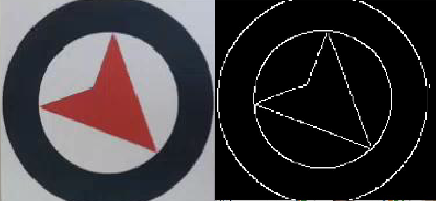
\includegraphics[width=4.5cm]{images/edgeDetect1.png}
		\caption{The edges are clear, shapes are easy to detect.}
	\end{subfigure}
	\begin{subfigure}[t]{5cm}
		\centering
		
\includegraphics[width=4.5cm]{images/edgeDetect2.png}
		\caption{The edges less clear, the background interferes}
	\end{subfigure}
	\begin{subfigure}[t]{5cm}
		\centering
		
\includegraphics[width=4.5cm]{images/edgeDetect3.png}
		\caption{The edges are too blurry, the quality is not good enough, shapes are not perceptible.}
	\end{subfigure}
	\caption{Edge detection on several crops of images more or less blurred and small with the same thresholds.}\label{fig:edgeDetection}
\end{figure}

\subsection{Metrics}

\paragraph{}
Quantifying the results is necessary in order to be able to compare the different methods. To that extent, the same metrics are used for all the algorithms tested. All the algorithms are tested on the test video - that has not been seen by the algorithm is a training phase is used. Is taken into account:
\begin{itemize}
    \item The number of detected logos. A logo is considered detected if $75\%$ of its screen time appearance is detected.
    \item The number of missed logos.
    \item The number of false positives, which is the number of objects detected that do not contain any logo.
    \item The time of execution to provide the \path{output.csv} file, in frame per second (fps). It is here measured on a local CPU, and provided with a standard deviation from an averaged measure every 30 images. This means that every 30 images, the time required to treat them is stored. This process is done multiple times on the same video with different starting frames, to reach a number of 1,000 samples of batch of 30 images computation time. These values are then converted to fps. The mean and standard deviation of this distribution is provided in the result tables.
\end{itemize}


\subsection{Results}
\paragraph{Accuracy}
Detecting the circles inside the picture reveals to be too difficult to calibrate; the results are poor (see \ref{fig:edgeResults}). A first focus on where to look before using computer vision is required for proper results. To that extent, deep learning is used.

\paragraph{Time of execution}
The time of execution is here very good, enough to be used on real time. The standard deviation shows that the complexity of the image impacts the treatment, even though the lowest quantile ($94.9 - 14.6 = 85.3$) remains more than enough to be used on the fly.

\begin{figure}
    \centering
        \begin{tabular}{c | c}
        Metric                  & Value \\
        \hline
        Detected logos          & 8 \\
        Missed logos            & 7 \\
        False positives         & 124 \\
        Time of execution (fps) & 94.9 (std = 14.6) \\
        \end{tabular}
    \caption{Metrics on algorithm using edge detection.}
    \label{fig:edgeResults}
\end{figure}


\section{Deep learning}

\paragraph{}
The deep learning approach relies on the use of a neural network already trained and adapted from the ImageNet and COCO classification problem, as described in the documentation of \href{https://github.com/tensorflow/models/tree/master/research/object_detection}{Google's Object Detection API} \cite{googleAPI}.
The idea is to retrain it with the local problem of our logo detection, and apply it frame by frame to detect boxes where the logo is likely to be.

\paragraph{}
The pros of that method is that it doesn't rely exactly on edge detection; it's more subtle, the features extracted from the frames are more diverse and more elaborate. It would also be adaptable to any object recognition, not only the logo problem, and this quite easily.

\paragraph{}
The cons are the fact that the model is very hard to explain; it's not trivial to determine why a box has been selected and one has not. This is a recurring problem with deep learning, even though a recent article on random forest applied to meta level training dataset is giving clues on interpretability  of hidden layers of a Deep CNN network \cite{interpretability}. Furthermore, the computation is bigger than with a simple edge detection. The training part can also be problematic; this model has been trained during 12 hours on a CPU but could give better results with a lower training rate/more computation power (no GPU available here).



\subsection{Dataset}

\subsubsection{Data augmentation}

\paragraph{}
The first thing to consider is the fact that a dataset to train the neural network. For this, data augmentation is used. A short video pretty clear of the logo is first shot, in order to have labeled frames zoomed on the logo. Then, several methods are used to have a dataset as diverse as possible. The dataset is not modified directly, but on the fly. The images, when regrouped in batches are applied some random transformation. The efficiency of simple techniques such as the one described in the section are still quite efficient and relevant \cite{dataAugmentation} 

\paragraph{}
By using enough batches, we can make sure that the probability of using all the possible combinations is pretty high. For example, if we apply $2$ transformation, let's call $A_i$ the event "the possibility i did not happen", $\forall i \in \llbracket 1~;~ n \rrbracket$ (with our configuration, there are only $n = 4$ possibilities). We denote $p_i$ the probability of $A_i$ (with our configuration, if we use the same probability $q = .5$, we have $\forall i \in \llbracket 1~;~ n \rrbracket, \ p_i = .75$). Then, for a batch of size $m$ we can the probability of not having used all the possibilities:
\begin{align*}
\Pr(\cap_{i=1}^{n} \overline{A_i}) &= 1 - \Pr(\cup_{i=1}^{n} A_{i})\\
&\geq 1 - \sum_{i=1}^{n} \Pr(A_i) \\
&\geq 1 - \sum_{i=1}^{n} p_i^{m} \\
\end{align*}
which is around $98\%$ for $m=20$ in this example. This is of course a simplistic situation. In the real use, the number of batch is very high compared to the value of each $p_i$, enough for this probability to remain in the same area - and be sure that the data augmentation was entirely exploited.

The transformations (see \ref{fig:dataAugmentationSample}) are used to make sure that the neural network has seen as many real life cases as possible. Here are what is used:
\begin{itemize}
    \item Random crops. The new image must remain big enough to have most of the logo on the frame. This simulates the logos that are partially cropped in the video.
    \item Random blurs. This simulates the movements of the camera.
    \item Random luminosity adjustments (brighter and darker).
    \item Random rotations, random horizontal and vertical flips.
    \item Random resizing.
\end{itemize}




\captionsetup[subfigure]{labelformat=simple, labelsep=period}
\begin{figure}
	\centering
	\begin{subfigure}[t]{2.5cm}
		\centering
		
\includegraphics[width=2.5cm]{images/logo.png}
		\caption{Original}
	\end{subfigure}
	\begin{subfigure}[t]{2.5cm}
		\centering
		
\includegraphics[width=2.5cm]{images/logoRandomRotation.png}
		\caption{Rotation}
	\end{subfigure}
	\begin{subfigure}[t]{2.5cm}
		\centering
		
\includegraphics[width=2.5cm]{images/logoLuminosity.png}
		\caption{Luminosity}
	\end{subfigure}
	\begin{subfigure}[t]{2.5cm}
		\centering
		
\includegraphics[width=2.5cm]{images/logoBlurred.png}
		\caption{Blurred}
	\end{subfigure}
	\begin{subfigure}[t]{2.5cm}
		\centering
		
\includegraphics[width=2.5cm]{images/logoRandomCrop.png}
		\caption{Cropped}
	\end{subfigure}
	\caption{Different transformations. They are not combined in this sample, which is the case in reality during the training.}\label{fig:dataAugmentationSample}
\end{figure}

\subsubsection{Train, validation and test set}

\paragraph{}
The dataset is then separated between a training set (70\%), a validation test(20\%) and a test set (10\%). The later is not touch during any part of the training, and used to judge the performances after training to make sure we're not overfitting. We move then forward to the training phase.

\subsection{Training}

\paragraph{}
The neural network used is a NaSNet architecture \cite{nasnet}. All the layers but the latest one is frozen, and the last one is replaced by a dense layer with one category output with a sigmoid activation function and a $.5$ threshold. Weight decay ($0.9$) is added to avoid overfitting; no dropout is used. A Nadam optimizer (Adam with a momentum component \cite{nadam}), with a learning rate at $0.001$, and a constant for numerical stability $\epsilon = 1$.

\paragraph{}
The training phase is performed on a CPU for 12 hours. This is definitely not optimal. A smaller or decreasing learning rate could give better results but requires too much computer power. The parameters could have been optimized in a better way but due to time and computation power constraint, the values of the literature have been used.

\begin{figure}
\centering
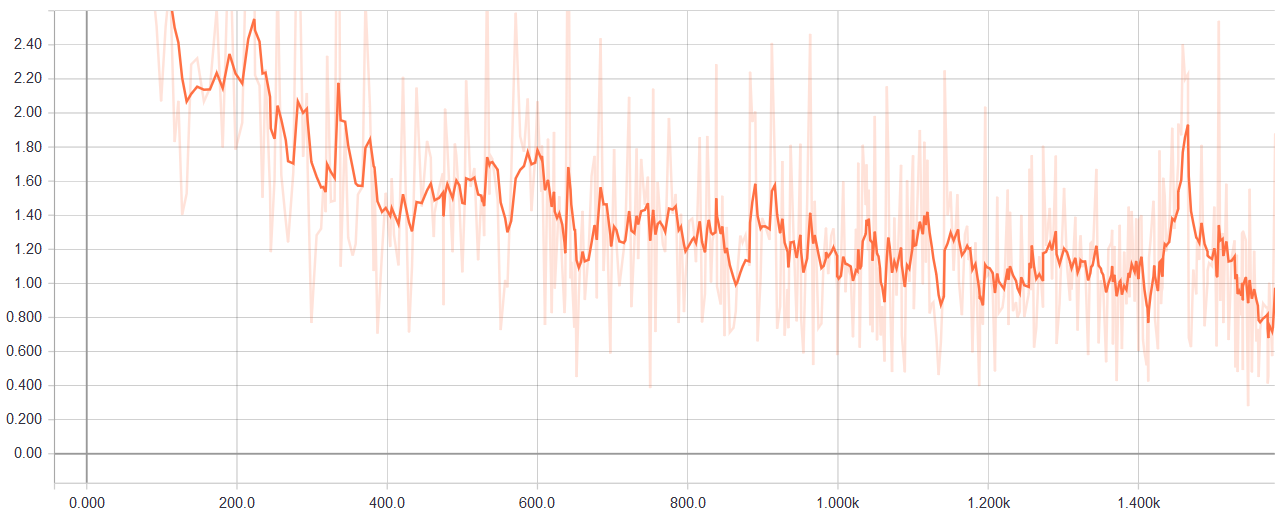
\includegraphics[width=15cm]{images/lossCurve.PNG}
\caption{\label{fig:loss}Loss evolution during the training. We can see that the training is not complete yet after less than 2,000 epochs.}
\end{figure}

\subsection{Results}

\paragraph{Accuracy}
The results from this methods are mixed. With this learning rate, we barely reach a loss below 1 (see \ref{fig:loss}), and the training could be ran for more epochs (around 10,000 would be better). That said, it performs already better than the simple edge/circle detection previously used (see \ref{fig:deepLearningResults}). It seems not to be that much bothered by the blurriness/bad luminosity of a few frames. There are however too many false positive that need to be reduced using another independent method. This is why another filter is added to the process.

\paragraph{Time of execution}
The time of execution is - as expected - worst than a simple edge analysis. It is however quite constant; it does not depend on the patterns of the figure, since the computation is rigorously the same whatever the image given. Given this, improving this could be quite easy, by for example skipping one out of two images, which would almost double the fps, reaching the real time constraint (24 fps).

\begin{figure}
    \centering
        \begin{tabular}{c | c}
        Metric                  & Value \\
        \hline
        Detected logos          & 14 \\
        Missed logos            & 1 \\
        False positives         & 43 \\
        Time of execution(fps)  & 12.4 (std = 0.7) \\
        \end{tabular}
    \caption{Metrics on algorithm using deep learning only.}
    \label{fig:deepLearningResults}
\end{figure}

\section{Deep learning and computer vision}

\paragraph{}
The technics used are design in order to detect false positives from true positives. The edge detection and shape recognition cannot be used since blurry images may be real logos. That's why others arguments are used.

\subsection{Format}
\paragraph{}
This one is pretty straightforward; the logos should be a square or not too far from it depending on the angle of the camera. this allows to remove a few false positive that have a ratio height/width above $2$ or bellow $1/2$. This filter is quite fast to apply (the complexity is $\mathcal{O}(1)$).

\subsection{Color distribution}
\paragraph{}
One thing that hasn't been used so far is the color distribution. Indeed, all the logo images should have - if the image is not too blurry - a peak in the color distribution for the background, the circle and the red quadrilateral. Unfortunately, this is not always the case, especially when the camera is moving too fast and the luminosity is not good enough.


\captionsetup[subfigure]{labelformat=simple, labelsep=period}
\begin{figure}
	\centering
	\begin{subfigure}[t]{10cm}
		\centering
		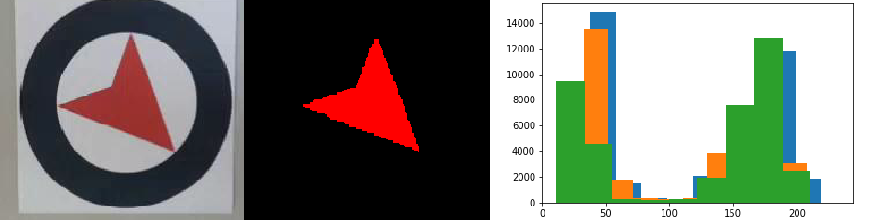
\includegraphics[width=9cm]{images/colorDistrib1.png}
		\caption{The distribution is neat, can be distinguished easily}
	\end{subfigure}
	\begin{subfigure}[t]{10cm}
		\centering
		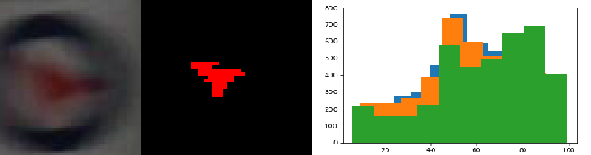
\includegraphics[width=9cm]{images/colorDistrib2.png}
		\caption{The distribution is more mixed; the percentage of red remains in the detectable area.}
	\end{subfigure}
	\caption{Images with detection of red and the RGB distribution of the colors.}\label{fig:colorDistrib}
\end{figure}
\paragraph{}
It is however possible to try to detect the amount of red in the picture, with what is considered red quite permissive ($red > 40$ and $red > \max(2*green, 2*blue)$). Indeed, a positive image should have at least a little bit of red, but the ratio $red\ pixels/number\ of\ pixels$ should not be more than a $25\%$ of the picture (number determined empirically by using positive and negative samples, see \ref{fig:colorDistrib}). This treatment is time consuming, the complexity being $\mathcal{O}(width*height)$. This could have been a feature detected by the neural network, but since we could not retrain the convolutions layers (size of training dataset + computation power), the feature are direcly used from the pretrained model - and not specific to our logo.

\subsection{Results}

\paragraph{Accuracy}
These treatments allows to get rid of a numerous amount of false positives (see \ref{fig:correctedDeepLearningResults}), without penalizing the true positive, the treatment remaining quite basic. The false positives left could even be improved by taking time into account; indeed, a lot of them are only detected on one frame (it's more difficult for a false positive to get through all the filters for several frames in a row), as discussed in the next section. 

\paragraph{Time of execution}
This treatment - especially the color check - makes the running time longer, since more computation is added to the already slow neural network. This depends on the number of boxed being treated, not constant, which explains the high standard deviation of the time of execution. Skipping images could be a solution, although to reach real time, an average of 3 our of 4 images would have to be skipped to reach 24 fps, and there is no guaranty that the algorithm would be on time - the treatment depends on the image.

\begin{figure}
    \centering
        \begin{tabular}{c | c}
        Metric                  & Value \\
        \hline
        Detected logos          & 17 \\
        Missed logos            & 1 \\
        False positives         & 18 \\
        Time of execution (fps) & 5.4 (std = 3.8) \\
        \end{tabular}
    \caption{Metrics on algorithm using deep learning and additional filters.}
    \label{fig:correctedDeepLearningResults}
\end{figure}


\captionsetup[subfigure]{labelformat=simple, labelsep=period}
\begin{figure}
	\centering
	\begin{subfigure}[t]{4cm}
		\centering
		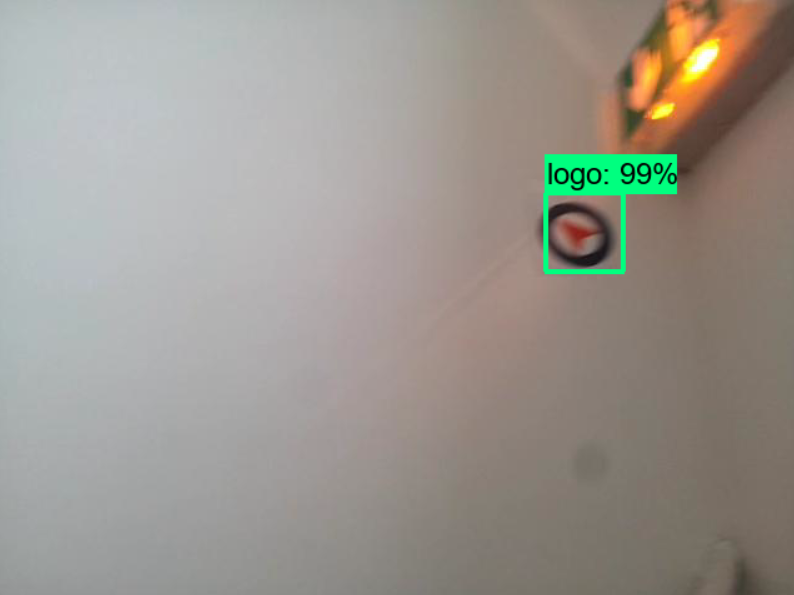
\includegraphics[width=4cm]{images/detection1.PNG}
	\end{subfigure}
	\begin{subfigure}[t]{4cm}
		\centering
		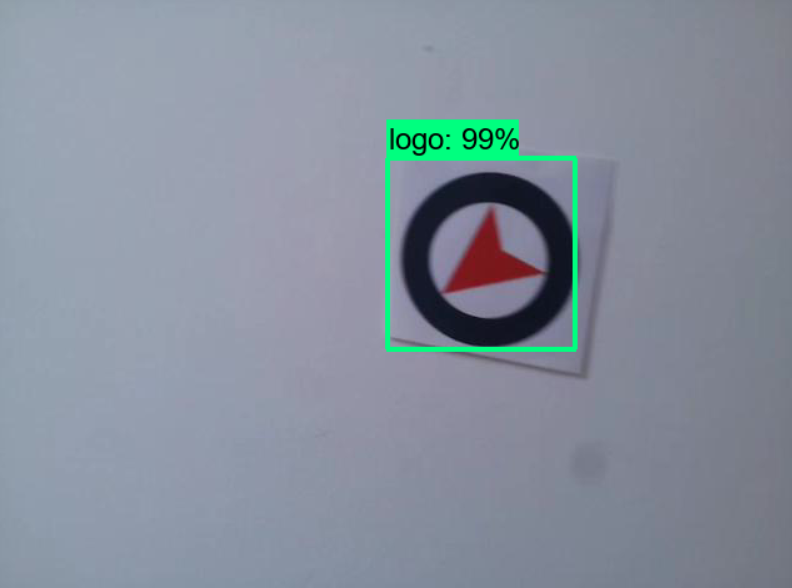
\includegraphics[width=4cm]{images/detection2.PNG}
	\end{subfigure}
	\begin{subfigure}[t]{4cm}
		\centering
		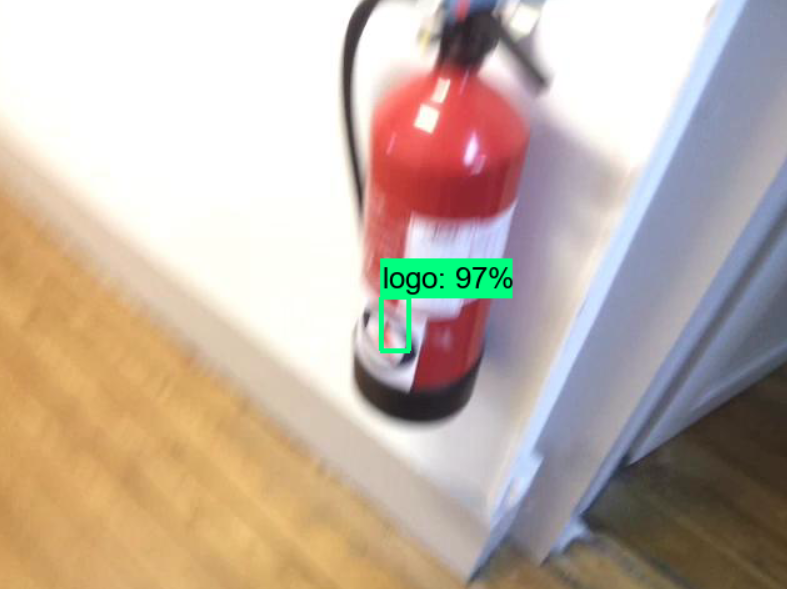
\includegraphics[width=4cm]{images/detection3.PNG}
	\end{subfigure}
	\begin{subfigure}[t]{4cm}
		\centering
		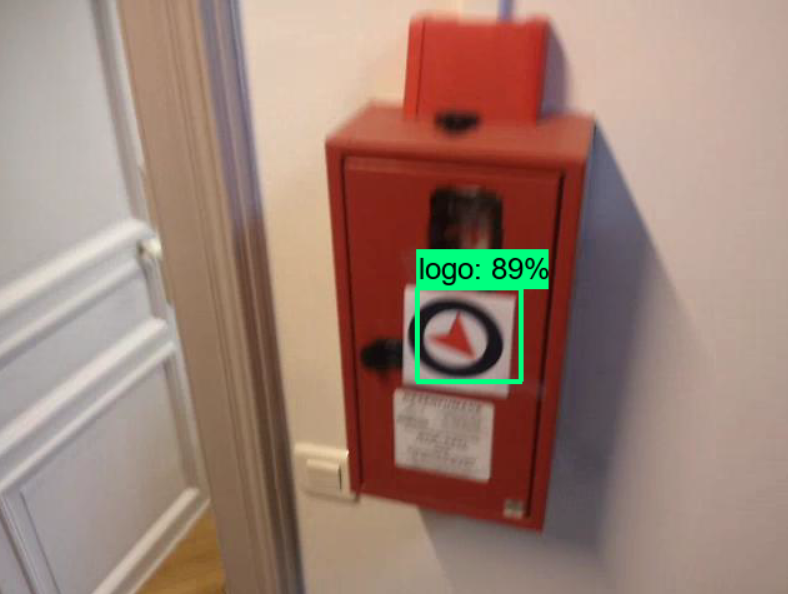
\includegraphics[width=4cm]{images/detection4.PNG}
	\end{subfigure}
	\caption{Sample of successful predictions on test images.}\label{fig:finalPredictionResults}
\end{figure}

\section{Next steps}\label{next-steps}

\subsection{Tracking}

\paragraph{}
The time factor is not used here. The frames are treated in an independent way, without any correlation nor order. A tracking algorithm could remedy this problem, such as using a K Nearest Neighbours Kalman filter \cite{kalman}. This method would use an already detected object, and try to follow the evolution from one frame to another. This is not trivial, since the camera is moving, the blurriness is definitely not helping the case.

\paragraph{}
The study of the trajectory could also be something used. Indeed, if we detect an object for a few frames, we can have an idea of where to look for coming up frame, and feeding the network with a restricted zone to identify the box (the normalization would be more effective that way). Extrapolating the position from a linear regression of the latest positions and cropping the image with a slightly bigger size than boxes previously detected could refine the new box detection.

\subsection{Offline Treatment}
\paragraph{}
If the treatment is done offline (or with a reasonable delay), knowing the "future" can really be useful in the detection of false positive and false negative. Indeed, an object not detected in between two frames where the object is can be recovered afterwards. The other way around, an object detected only for one frame with no continuity could be removed: if a logo is detected for only one frame (in time), we can be suspicious about this detection.

\subsection{Real time treatment}
\paragraph{}
The model used here does not allow the real time processing, at least on CPU. A few amelioration could improve this, such as jumping a few frames and extrapolating the position of the logos in the middle. Otherwise, lighter network could be used, such as the YOLO \cite{yolo} have better performances (reaching 45fps or 155fps for the light version); this is however always a trade off between speed and accuracy.

\section{Conclusion}
\paragraph{}
This project measures several methods to detect the Sysnav logo in a video. There are still many possible improvements to do. The cons of the last methods used include the fact that it is easy to modify the searched object, and to play with the filters post detection with deep learning.

\paragraph{}
The classic trade off between speed and accuracy is encountered as well, and can be more exploited within operational applications; treating the video in a semi-online way (online but with a delay of a few frames) could improve the correction of false positives with the treatments suggested in the section \ref{next-steps}.


\begin{thebibliography}{9}
\bibitem{canny} 
John Canny. 
\textit{A Computational Approach to Edge Detection}. 
1986.

\bibitem{googleAPI}
Huang J, Rathod V, Sun C, Zhu M, Korattikara A, Fathi A, Fischer I, Wojna Z,
Song Y, Guadarrama S, Murphy K.
\textit{Speed/accuracy trade-offs for modern convolutional object detectors}.
2017.

\bibitem{nadam}
Timothy Dozat.
\textit{Incorporating Nesterov Momentum into Adam}.
2015.
 
\bibitem{kalman} 
Dan Iter, Jonathan Kuck, Philip Zhuang.
\textit{Target Tracking with Kalman Filtering, KNN and LSTMs}.
2016.

\bibitem{yolo}
Joseph Redmon, Santosh Divvala, Ross Girshick, Ali Farhadi.
\textit{You Only Look Once: Unified, Real-Time Object Detection}.
2016.
 
\bibitem{dataAugmentation}
Jason Wang; Luis Perez.
\textit{The Effectiveness of Data Augmentation in Image Classification using Deep Learning}.
2017.
 
\bibitem{interpretability}
Xuan Liu, Xiaoguang Wang, Stan Matwin.
\textit{Interpretable Deep Convolutional Neural Networks via Meta-learning}.
2018.

\bibitem{nasnet} 
Barret Zoph, Vijay Vasudevan, Jonathon Shlens, Quoc V. Le.
\textit{Learning Transferable Architectures for Scalable Image Recognition}.
2018.
\end{thebibliography}




\end{document}
